\documentclass[10pt,twocolumn,letterpaper]{article}

\usepackage{cvpr}
\usepackage{times}
\usepackage{epsfig}
\usepackage{graphicx}
\usepackage{amsmath}
\usepackage{amssymb}
\usepackage[ruled,vlined]{algorithm2e}
\usepackage[noabbrev,capitalize]{cleveref}
\usepackage{listings}
\lstset{language=C++}


\usepackage{url}

% Include other packages here, before hyperref.

% If you comment hyperref and then uncomment it, you should delete
% egpaper.aux before re-running latex.  (Or just hit 'q' on the first latex
% run, let it finish, and you should be clear).
%\usepackage[pagebackref=true,breaklinks=true,letterpaper=true,colorlinks,bookmarks=false]{hyperref}

\cvprfinalcopy % *** Uncomment this line for the final submission

\def\cvprPaperID{****} % *** Enter the CVPR Paper ID here
\def\httilde{\mbox{\tt\raisebox{-.5ex}{\symbol{126}}}}

% Pages are numbered in submission mode, and unnumbered in camera-ready
\ifcvprfinal\pagestyle{empty}\fi
\begin{document}

%%%%%%%%% TITLE
\title{Project 2: K-Means Clustering}

\author{Marco Di Rienzo\\
{\tt\small marco.dirienzo@stud.unifi.it}
% For a paper whose authors are all at the same institution,
% omit the following lines up until the closing ``}''.
% Additional authors and addresses can be added with ``\and'',
% just like the second author.
% To save space, use either the email address or home page, not both
}

\maketitle
\thispagestyle{empty}

%%%%%%%%% ABSTRACT
\begin{abstract}
	The goal of this paper is to parallelize the K-Means Clustering algorithm and analyze the performance gain with respect to the sequential version.\\
	One parallel versions has been created using the OpenMP framework and another using CUDA to run on the GPU.\\
	The performance gain is measured in terms of $\text{speed-up}=\frac{\text{sequential time}}{\text{parallel time}}$.
\end{abstract}

%%%%%%%%% BODY TEXT
\section{Introduction}
Both the sequential and the parallel version of the algorithm have been implemented in C++, the parallel ones using the OpenMP framework and CUDA C.\\
The dataset used to perform the tests is composed of 100,000 points of 2 dimensions and has been generated with the \texttt{make\_blobs} function of \textit{sklearn}.\\
Since the algorithm involves an initial random choice between the dataset points, a fixed seed has been imposed to both versions to yield comparable results.

\section{Pseudocode}
The implemented algorithm has the following pseudocode:
\begin{algorithm}
	\SetAlgoLined
	\KwData{$k$, $max\_iterations$, $observations$}
	\KwResult{$centroids$, $labels$}
	1. Select $k$ random $observations$ as starting $centroids$\;
	\While{not $max\_iterations$}{
		\ForEach{$observation$}{
			2. Compute the distance between each $centroid$ and $observation$\;
			3. Assign $observation$ to closest $centroid$\;
		}
		4. Compute new $centroids$ (mean of $observations$ in a cluster)\;
	}
	\caption{K-Means Clustering}
	\label{pseudocode}
\end{algorithm}

\section{Algorithm nature} \label{nature}
The algorithm lends itself very well to parallelization because the main loop (steps 2. and 3. of \cref{pseudocode}) is embarrassingly parallel, i.e. every iteration is independent from one another. What this means is that observations (points of the dataset) can simply be distributed among any number of threads while not having to worry about communication whatsoever.

\section{Languages and frameworks}
The codebase of the project has been written in C++. Python has been used to analyze the results.\\
One parallel version has been created using the framework OpenMP, which allows the code to remain pretty much the same while distributing the workload among threads, instructed by the use of directives. This framework is ideal in this case because the only section to parallelize is the \textit{foreach} of \cref{pseudocode} which as said in \cref{nature} is embarrassingly parallel, and it can be done with a single directive (and some ad-hoc reduction functions).\\
The other one was made with CUDA C, which allows even more parallelization since GPUs are capable of managing thousands of threads.

\section{Sequential implementation} \label{seq_imp}
The sequential implementation is basically a C++ translation of the pseudocode in \cref{pseudocode}, with some nuances: 
\begin{enumerate}
	\item Observations and centroids are organized as Array of Structures to improve the alignment with cache lines and benefit of the memory bursts when accessing the various coordinates.
	\item Step 4. is partially executed in the for loop, in particular the sum required to compute the mean is updated as soon as a point is assigned to a centroid. This avoids having to loop again on every observation, and is also perfectly compatible with the later parallelization.
\end{enumerate}

\section{Parallel implementation}
Parallelizing step 1. makes no sense since $k$ is usually small and there's practically no computation required to choose random points from the given ones.\\
The best we can do with step 4. is making each thread update a partial sum as soon as a point is assigned to a centroid, which is what we already explained in \cref{seq_imp}; the actual mean computation is not a parallelizable problem.\\
The embarrassingly parallel section of the algorithm is the for loop.
\subsection{OpenMP}
The directive \textbf{\#pragma omp parallel for} allows splitting observation indices among threads, so that each one will be assigned a different subset of the dataset.\\
Since the assignments of observations to clusters are independent from one another, no synchronization is required.\\
However, since a partial sum of points in a cluster is maintained in each thread, a final reduction is needed to extract the total sum and be able to compute the mean; this is accomplished with the directive \textbf{\#pragma omp declare reduction(...)} which allows to specify a reduction function to conglomerate the data of each thread.\\
Custom reduction functions have been created to deal with the structures used in the program.
\subsection{CUDA}
Since GPUs' threads context switch is negligible, each thread is assigned a single observation, this way, the for loop can be removed and so the maximum parallelization possible is achieved.\\
Observations and initial centroids are copied from the host to the device \textbf{global memory}, and also arrays to store new centroids, the number of points per cluster and point labels are created; centroids are then pulled to \textbf{shared memory} to improve access time since they have to be read by every thread.\\
Inside a thread, its point is compared with every centroid and the resulting label is written in the global memory array. The points per cluster and new centroids arrays are atomically increased, so no manual synchronization is required.\\
After the kernel completes, every thread of the grid is synchronized so final values of sum of points in a cluster and the number of points per cluster are available.
Another kernel is launched to compute the new centroids directly on the device, so to avoid copying arrays back to host at every iteration.\\
Only when final centroids are computed, the centroids coordinates and point labels are retrieved from the device and saved.\\

\section{Tests}
Every test has been carried out on a CPU Intel Core i5-4670 (4-core) and a GPU Nvidia GeForce GTX 770 (compute capability 3.0).\\
The dataset used to perform the tests was generated with the \texttt{make\_blobs} function of \textit{sklearn} and is composed of 100,000 elements of 2 dimensions.\\
The purpose of these tests was the measurement of the speed-up of the parallel implementations of the algorithm against the sequential one.\\
Wall-clock time was measured by C++ standard functions of the \texttt{<chrono>} library.\\
Each time the parallel and sequential version were given the same seed to make the initial random choice of centroids consistent between executions.\\
\subsection{OpenMP}
The parallel program was run with varying number of threads with the purpose to find the optimum value.\\
Time results and resulting speed-up of the trials for OpenMP are shown in \cref{table:speedup}, and also graphically in \cref{fig:speedup}, it can be seen that the speed-up grows sub-linearly to the best execution time, achieved with \textbf{4 threads}, that is the exact number of CPU cores. This is because with less threads obviously the amount of work per thread is greater and thus more time is required to complete.\\ With more threads, it's true that each one has less points to process, but since only 4 cores are available, only 4 threads can be executed simultaneously, and there's also the overhead of switching threads in and out of the processors.\\
This is especially true in our case since each thread doesn't need to wait for any resources and thus there's no advantage in having more threads in the queue.\\
In fact, with 5 threads and beyond the speed-up remains constant at about 2.5.
\subsection{CUDA}
According to the \textbf{CUDA Occupancy Calculator} the number of threads per block was set to 128; the corresponding number of blocks is $\lceil \frac{N_{points}}{128} \rceil$.\\
Tests have been made with increasing dataset size to appreciate the scaling of the various parallelization methods.\\
Results are shown in \cref{table:time_to_size}, and also graphically in \cref{fig:time_to_size}, it can be seen that the sequential implementation scales linearly to dataset size, while the parallel ones scale sub-linearly, with CUDA gaining more and more advantage as the size increases due to the maximum parallelization of a single point per thread.\\

\begin{table*}[h]
	\centering
	\begin{tabular}{|l|c|c|c|c|c|c|c|c|c|c|}
		\hline
		N. of Threads        & 1    & 2    & 3    & 4    & 5    & 6    & 7    & 8    & 9    & 10   \\ \hline
		Time Sequential (ms) & 275  &      &      &      &      &      &      &      &      &      \\ \hline
		Time Parallel (ms)   & 272  & 136  & 94   & 78   & 130  & 114  & 102  & 111  & 119  & 110  \\ \hline
		Speed-up             & 1.01 & 2.02 & 2.93 & 3.53 & 2.12 & 2.41 & 2.70 & 2.48 & 2.31 & 2.50 \\ \hline
	\end{tabular}\\
	\bigskip
	\caption{Execution time (milliseconds) and resulting speed-up of sequential vs OpenMP parallel implementation, with number of threads from 1 to 10.}
	\label{table:speedup}
\end{table*}
\begin{figure*}[h]
	\begin{center}
		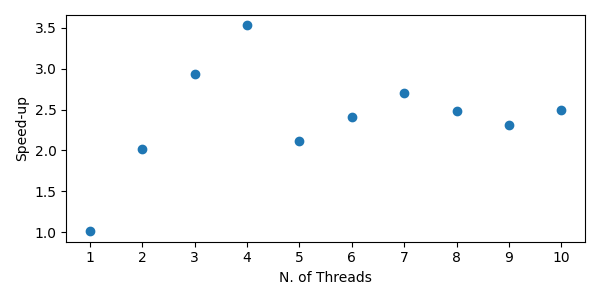
\includegraphics[width=\textwidth]{img/speedup_OMP.png}
	\end{center}
	\caption{Plot of OpenMP speed-up values against number of threads displayed in \cref{table:speedup}.}
	\label{fig:speedup}
\end{figure*}

\clearpage
\begin{table*}[h]
	\centering
	\begin{tabular}{|l|c|c|c|c|c|c|c|c|c|c|}
		\hline
		Dataset size (1e4)   & 1    & 2    & 3    & 4    & 5    & 6    & 7    & 8    & 9    & 10   \\ \hline
		Time Sequential (ms) & 27 & 55 & 76 & 106 & 132 & 152 & 186 & 207 & 246 & 275  \\ \hline
		Time OpenMP (ms)     & 7 & 17 & 28 & 32 & 41 & 49 & 61 & 67 & 77 & 78  \\ \hline
		Time CUDA (ms)       & 4 & 5 & 8 & 8 & 10 & 13 & 13 & 16 & 18 & 19 \\ \hline
		Speed-up OpenMP   & 3.86 & 3.24 & 2.71 & 3.31 & 3.22 & 3.1 & 3.05 & 3.09 & 3.19 & 3.53  \\ \hline
		Speed-up CUDA   & 6.75 & 11.0 & 9.5 & 13.25 & 13.2 & 11.69 & 14.31 & 12.94 & 13.67 & 14.47  \\ \hline
	\end{tabular}\\
	\bigskip
	\caption{Execution time (milliseconds) and resulting speed-up of sequential vs OpenMP vs CUDA parallel implementation, with dataset size from $10^4$ to $10^5$.}
	\label{table:time_to_size}
\end{table*}
\begin{figure*}[h]
	\begin{center}
		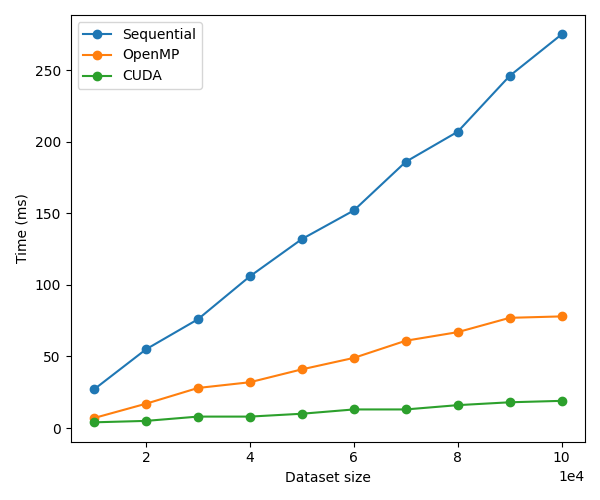
\includegraphics[width=0.8\textwidth]{img/time_to_size.png}
	\end{center}
	\caption{Plot of execution time against dataset sizes displayed in \cref{table:time_to_size}.}
	\label{fig:time_to_size}
\end{figure*}

\end{document}
